\lesson{17}{16/04/2020}Now, we have all we need to find the generic B\&S formula with stochastic interest rate. For a call option
\begin{equation}
    \pay_T = (S(T)-K)^+
\end{equation}
so the price is 
\begin{align}\label{stocrcall}
    \notag\call_t &= \expect_t\left[(S(T)-K)^+e^{\int_t^T r_s\,\dd s}\right]\\
    &=
    \notag\expect_t\left[e^{-\int_t^T r_s\,\dd s}S(T)\mathds{1}_{S_T\ge K}\right] - K\expect_t\left[e^{-\int_t^T r_s\,\dd s}\mathds{1}_{S_T\ge K}\right]\\
    \overset{(a)}&{=}
    \notag\expect_t\left[e^{-\int_t^T r_s\,\dd s}S(t)e^{-\int_t^T r_s\,\dd s  - \frac{\sigma^2}{2}(T-t)+\sigma(W_T^{\Qmeas}-W_t^{\Qmeas})}\mathds{1}_{S_T\ge K}\right] - KB(t,T)\expect_t\left[\mathds{1}_{S_T\ge K}\right]\\
    &=
    \notag S(t)\expect_t\left[e^{-\frac{\sigma^2}{2}(T-t)+\sigma(W_T^{\Qmeas}-W_t^{\Qmeas})}\mathds{1}_{S_T\ge K}\right] - KB(t,T)\Qmeas^T(\mathds{1}_{S_T\ge K})\\
    &= 
    \notag S(t)\mathbb{E}^{\Qmeas^s}_t[S_T\ge K] - KB(t,T)\Qmeas^T(S_T\ge K) \\
    &= 
    S(t)\Qmeas^s(S_T\ge K) - KB(t,T)\Qmeas^T(S_T\ge K)
\end{align}
Where in (a) we use the explicit expression for $S(T)$ and in order to split the second expected value we use the zero coupon bond as numéraire. In (b) we use the change of measure $\Qmeas\to\Qmeas^s$ associated to $s$'s numéraires, with corresponding Radon-Nikodym derivative
\begin{equation}
    \eval{\frac{\dd\Qmeas^s}{\dd\Qmeas}}_t = \dfrac{S(T)}{\expect[S(T)]}
\end{equation}
Eq. \eqref{stocrcall} is the analogous of the B\&S formula in the general case with stochastic interest rate (in the standard B\&S formula we would have the gaussian CDFs). However, in principle we don't know the distributions of $S(t)$ under $\Qmeas^s$ and $\Qmeas^T$. \\
Let's consider the particular case in which the volatility of the process $S(t)/B(t,T)$ is deterministic. In order to deal with the volatility we need to write the dynamics of the process in terms of a geometric Brownian motion-like form:
\begin{equation}
    \dfrac{\dd\left(\frac{S(t)}{B(t,T)}\right)}{\frac{S(t)}{B(t,T)}} = (\dots)\,\dd t + \sigma\,\dd W
\end{equation}
As usual, if we introduce the auxiliary process 
\begin{equation}
    Z(t) \coloneqq \frac{S(t)}{B(t,T)}
\end{equation}
we have that:
\begin{equation}
    \dfrac{\dd Z(t)}{Z(t)} = (\dots)\,\dd t + \sigma_Z(t)\,\dd W^{\Qmeas}
\end{equation}
where $\sigma_Z$ is deterministic. Notice that the denominator of $Z(t)$ is a possible numéraire. In particular, if we set the dynamics of $Z(t)$ under probability measure associated to $B$, i.e. the forward measure, then $Z(t)$ becomes a martingale. So, we have that:
\begin{equation}
    \dfrac{\dd Z(t)}{Z(t)} = 0\,\dd t + \sigma_Z(t)\,\dd W^{\Qmeas^T}
\end{equation}
The solution at time $T$ is:
\begin{align}
    Z(T) &= Z_0\exp{{-\frac{1}{2}\int_0^T\norm{\sigma_Z(t)}^2\,\dd t - \int_0^T\sigma_Z(t)\cdot\dd W^{\Qmeas^T}}} \\
    \overset{(a)}&{=}
    \dfrac{S(0)}{B(0,T)}\exp{{\mathcal{N}\left(-\frac{1}{2}\int_0^T\norm{\sigma_Z(t)}^2\,\dd t; \int_0^T\norm{\sigma_Z(t)}^2\dd t\right)}}
\end{align}
where in (a) we used the fact that if $\sigma_Z$ is deterministic then $\int_0^T\sigma_Z\cdot\dd W^{\Qmeas^T}$ is gaussian (martingale) with expected value equal to zero. With that being said, the first term represents only a shift in the expected value. The variance of the Gaussian comes from the \emph{Itô's isometry}\footnote{Itô's isometry states that if $H\in\mathcal{H}$, then
\begin{equation}\label{itoes}
    \mathbb{E}\left[\left(\int_0^T H_s\,\dd W_s\right)^2\right] = \mathbb{E}\left[\left(\int_0^T H_s^2 \,\dd s\right)^2\right] \tag{$\diamond$}
\end{equation}
Then:
\begin{equation*}
    \Var\left(\int_0^T\sigma_Z(s)\cdot\dd W^{\Qmeas^T}\right) = \mathbb{E}\left[\left(\int_0^T\sigma_Z(s)\cdot\dd W^{\Qmeas^T}\right)^2\right] 
    \overset{\eqref{itoes}}{=} \mathbb{E}\left[\int_0^T\norm{\sigma_Z(s)}\,\dd s\right] 
    = 
    \int_0^T\norm{\sigma_Z(s)}\,\dd s
\end{equation*}
In other words, the relationship between deterministic and stochastic integrals is not linear, but quadratic.}.\\
Now, we can compute the price of the call \eqref{stocrcall}:
\begin{align}
    \call_T &= S(t)\hlc{mypink}{\Qmeas^s(S(T)> K)} - KB(t,T)\hlc{mylightblue}{\Qmeas^T(S(T)> K)}
\end{align}
By using the fact that $B(T,T)=1$, we can write:
\begin{equation*}
    \hlc{mylightblue}{\Qmeas^T(S(T)> K)} = \Qmeas^T\left(\dfrac{S(T)> K}{1}\right) = \Qmeas^T\left(\dfrac{S(T)> K}{B(T,T)}\right) = \Qmeas^T(Z(T)> K) = \Phi(d_2)
\end{equation*}
with
\begin{equation}
    d_2 = \dfrac{\ln\dfrac{S(t)}{B(t,T)K}-\frac{1}{2}\int_t^T\norm{\sigma_Z}^2\,\dd s}{\sqrt{\int_t^T\norm{\sigma_Z}^2\,\dd s}}
\end{equation}
Notice that if we consider a constant interest rate we have $B(t,T)=e^{-r(T-t)}$ and we recover the B\&S formula for $d_2$.\\ %vedi notes
Then, we can write:
\begin{equation}\label{Qs}
    \hlc{mypink}{\Qmeas^s(S(T)\ge K)} = \Qmeas^s\left(\frac{1}{S(T)}\le\frac{1}{K}\right) = \Qmeas^s\left(\frac{B(T,T)}{S(T)}\le\frac{1}{K}\right) = \Qmeas^s\left(\frac{1}{Z(T)}\le\frac{1}{K}\right)
\end{equation}
where 
\begin{equation}
    \frac{1}{Z(T)} = \frac{B(T,T)}{S(T)} = \Qmeas^S-martingale
\end{equation}
so that
\begin{equation}
    \dfrac{\dd \frac{1}{Z(T)}}{\frac{1}{Z(t)}} = 0\,\dd t + \sigma_{1/Z}\,\dd W^{\Qmeas^s}(t) = -\sigma_Z \,\dd W^{\Qmeas^s}(t) %"last time we saw that the volatility of 1/BrowMotion is -sigma_BrowMotion" ???
\end{equation}
This equation is a Brownian motion differential equation, which has solution:
\begin{align}
    \frac{1}{Z(T)} &= \frac{1}{Z(0)}\exp{{-\frac{1}{2}\int_0^T\norm{\sigma_Z(t)}^2\,\dd t - \int_0^T\sigma_Z(t)\cdot\dd W^{\Qmeas^T}}} \\
    &= 
    \dfrac{B(0,T)}{S(0)}\exp{{\mathcal{N}\left(-\frac{1}{2}\int_0^T\norm{\sigma_Z(t)}^2\,\dd t; \int_0^T\norm{\sigma_Z(t)}^2\dd t\right)}}
\end{align}
Now we can come back to eq. \eqref{Qs}:
\begin{equation}
    \hlc{mypink}{\Qmeas^s(S(T)\ge K)} = \Qmeas^s\left(\frac{1}{Z(T)}\le\frac{1}{K}\right) = \Phi(d_1)
\end{equation}
where
\begin{equation}
    d_1 = d_2 + \sqrt{\int_0^T\norm{\sigma_Z(t)}^2\dd t}
\end{equation}
Finally, we conclude that, if the volatility of the process $S(t)/B(t,T)$ is constant, the price of a call option is:
\begin{equation}\label{stocrcall1}
    \call_t = S(t)\Phi(d_1) - KB(t,T)\Phi(d_2)
\end{equation}
Eq. \eqref{stocrcall1} has the same shape as the B\&S formula and the only difference is in the expression of $d_1$ and $d_2$.\\ However, we have still to specify the dynamics of the interest rate. % end pt. 1
\begin{example}{Vašíček model}{}{}
    The Vašíček model (1979) is the first model that described the evolution of interest rates. It considers the \emph{instantaneous (spot) interest rate} $r_t$ corresponding to the infinitesimal interval $[t,t+\dd t]$ and the main assumption is that:
    \begin{equation}\label{vasmodel}
        \dd r_t = (a-br_t)\dd t + \sigma_r\dd W^{\Qmeas}(t)
    \end{equation}
    where $W^{\Qmeas}$ is a Brownian motion (under the risk neutral probability measure $\Qmeas$) that models the continuous inflow of randomness into the system. The typical parameters can be quickly characterized as follows:
    \begin{itemize}
        \item $b>0$ represents the ``long term mean level", i.e. all future trajectories of $r$ will evolve around a mean level $b$ in the long run;
        \item $a>0$ characterizes the ``speed of reversion", i.e.  the velocity at which such trajectories will regroup around $b$ in time;
        \item $\sigma_r>0$ represents the ``instantaneous volatility", which measures instant by instant the amplitude of randomness entering the system. Higher $\sigma_r$ implies more randomness.
    \end{itemize}
    The starting interest rate $r_0$ is not observable, since it is instantaneous (the short interest rate is an abstraction). This mean that in this model the interest rate is not tradable.\\
    Let's see why this is the dynamics. If we suppose that $\sigma_r=0$ (deterministic dynamics), then eq. \eqref{vasmodel} becomes:
    \begin{equation}\label{rdyn}
        \dd r_t = (a-br_t)\dd t \qquad\Rightarrow\qquad \Dot{r}_t = b\left(\frac{a}{b}-r_t\right)
    \end{equation}
    The solution $r_t$ of this differential equation will have an exponential behavior with convergence to the asymptotic value $r_{\infty}$. The presence of Brownian noise induces some fluctuations around the deterministic trajectory, as shown in Figure \ref{fig:vasicek}.
    \begin{center}\label{fig:vasicek}
        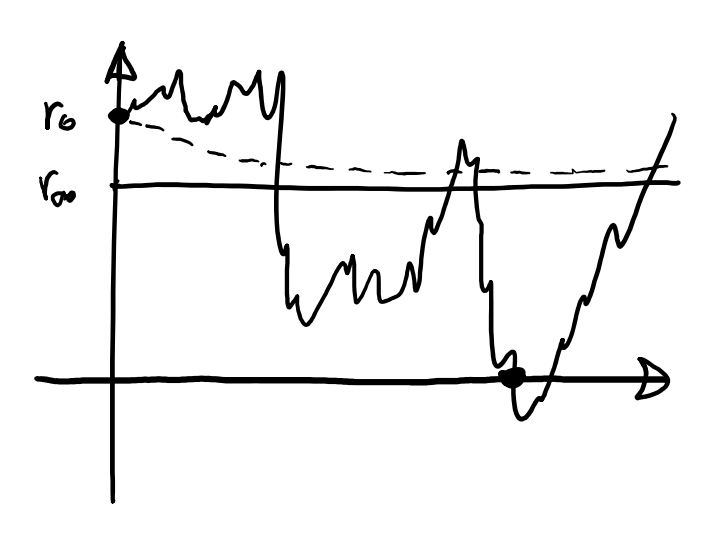
\includegraphics[scale=0.3]{fig/tmp/fig30.png}
        \captionof{figure}{Dynamics of the interest rate $r_t$ with initial condition $r_0$ and asymptotic value $r_{\infty}$.}
    \end{center}
    In order to find the solution of eq. \eqref{rdyn}, we consider the following differential:
    \begin{align}
        \notag \dd(r_te^{bt}) &= e^{bt}\dd r_t + r_t\dd e^{bt} \\
        &= 
        \notag e^{bt}(a-br_t)\dd t + e^{bt}\sigma_r \dd W^{\Qmeas} + br_te^{bt}\dd t \\
        &= 
        ae^{bt}\dd t + \sigma_r e^{bt} + \sigma_r e^{bt} \dd W^{\Qmeas}(t)
    \end{align}
    Integrating from 0 to $t$, we get:
    \begin{align}
        r_t e^{bt} - r_0 = \frac{a}{b}(e^{bt}-1) + \sigma_r \int_0^t e^{bs}\,\dd W^{\Qmeas}(s)
    \end{align}
    from which:
    \begin{equation}
        r_t = r_0e^{-bt} + \frac{a}{b}(1-e^{-bt}) + \sigma_r \int_0^t e^{-b(t-s)}\,\dd W^{\Qmeas}(s)
    \end{equation}
    It is very simple to check that $e^{-b(t-s)}\in\mathbb{H}$, so the integral is a martingale, in particular a gaussian variable $\mathcal{N}\left(0;\sigma_r^2\int_0^te^{-2b(t-1)}\,\dd s\right) = \mathcal{N}\left(0;\frac{\sigma^2_r}{2b}\left(1-e^{-2bt}\right)\right)$. The deterministic part results in a shift in the mean, so we end up with:
    \begin{equation}
        r_t \sim \mathcal{N}\left(r_0 + \frac{a}{b}(1-e^{-bt});\frac{\sigma^2_r}{2b}\left(1-e^{-2bt}\right)\right)
    \end{equation}
    It turns out that in the Vašíček model the interest rate is a gaussian variable. In particular, $\Qmeas(r_t<0)>0$: in the past it represented a problem because the short interest rate was supposed to be strictly positive. This convention was dropped after the 2008 crisis.\\
    The simpler product to be priced in this framework is the zero-coupon bond. We would like to check if the volatility of the process $S(t)/B(t,T)$ is deterministic or not. In order to do that, we try to limit ourselves to the minimal needed information about $B(t,T)$. \\
    If we fix $s\ge t$ as starting point, we have:
    \begin{equation}
        r_s = r_te^{-b(s-t)} + \frac{a}{b}(1-e^{-b(s-t)}) + \sigma_r \int_t^s e^{-b(s-u)}\,\dd W^{\Qmeas}(u)
    \end{equation}
    The price of the zero-coupon bond is given by:
    \begin{align}\label{B}
        B(t,T) = \expect_t\left[e^{-\int_t^Tr_s\,\dd s}\right]
    \end{align}
    First, we compute the integral:
    \begin{align}
        \notag -\int_t^Tr_s\,\dd s &= -r_t\int_t^T e^{-b(s-t)}\,\dd s - \frac{a}{b}\int_t^T(1-e^{-b(s-t)})\,\dd s - \\
        &\qquad\qquad\qquad 
        - \sigma_r\int_t^T \left(\int_t^s e^{-b(s-u)}\,\dd W^{\Qmeas}_u\right)\dd u
    \end{align}
    The first two integrals are easy to compute, while the third is feasible thanks to the stochastic Fubini theorem. Since there is not dependence on the interest rate, the third integral will result in a Gaussian variable $\mathcal{N}(0;\Sigma^2)$ with zero mean and variance given by the Itô's isometry. If we solve the first integral and we consider the second integral as a shift in the mean we end up with:
    \begin{align}
        -\int_t^Tr_s\,\dd s = -\dfrac{r_t}{b}(e^{-b(T-t)}-1) - \mathcal{N}(m;\Sigma^2)
    \end{align}
    Plugging in eq. \eqref{B} we get:
    \begin{equation}
        B(t,T) = \expect_t\left[e^{-\frac{r_t}{b}(e^{-b(T-t)}-1)}e^{-\mathcal{N}(m;\Sigma^2)}\right]
    \end{equation}
    By Itô, the dynamic of the zero-coupon bond is:
    \begin{align}
        \notag\dd B(t,T) &= \pdv{B(t,T)}{t}\,\dd t + \pdv{B(t,T)}{r_t}\,\dd r_t + \frac{1}{2}\pdv[2]{B(t,T)}{r_t}\,\dd\expval{r}_t \\
        \overset{\eqref{vasmodel}}&{=}
        \notag(\dots)\,\dd t + B(t,T)\frac{e^{-b(T-t)}-1}{b}((a-br_t)\dd t + \sigma_r\,\dd W^{\Qmeas}) \\
        \overset{(a)}&{=} 
        (\dots)\,\dd t + B(t,T)\frac{e^{-b(T-t)}-1}{b}\sigma_r\,\dd W^{\Qmeas}
    \end{align}
    and then:
    \begin{align}\label{dbb}
        \frac{\dd B(t,T)}{B(t,T)} = (\dots)\,\dd t + \frac{e^{-b(T-t)}-1}{b}\sigma_r\,\dd W^{\Qmeas}
    \end{align}
    So, the volatility of $B(t,T)$ in the Vašíček model is given by:
    \begin{equation}
        \sigma_B = \frac{e^{-b(T-t)}-1}{b}
    \end{equation}
    Now, if we consider the ratio:
    \begin{equation}
        \frac{\dd\frac{S(t)}{B(t,T)}}{\frac{S(t)}{B(t,T)}} = \hlc{mypink}{\left(\sigma-\sigma_r\frac{e^{-b(T-t)}-1}{b}\right)\dd W^{\Qmeas}} + (\dots)\,\dd t
    \end{equation}
    we have that the highlighted term is deterministic, so it is possible to find the B\&S formula for the price of a call in the Vašíček model. If we denote
    \begin{equation}
        \sigma-\sigma_r\frac{e^{-b(T-t)}-1}{b} \equiv \sigma_z
    \end{equation}
    then we have
    \begin{align} 
        d_1 = \dfrac{\ln\dfrac{S(t)}{B(t,T)K}-\frac{1}{2}\int_t^T\norm{\sigma_Z}^2\,\dd s}{\sqrt{\int_t^T\norm{\sigma_Z}^2\,\dd s}}
    \end{align} % d_1 o d_2?? prima questo era d_2
    Notice that, as expected, the zero-coupon bond becomes deterministic at maturity (it gives one unit of money), in fact for $t=T$ eq. \eqref{dbb}:
    \begin{equation*}
        \frac{\dd B(t,T)}{B(t,T)} = (\dots)\,\dd t + \frac{e^{-b(T-T)}-1}{b}\sigma_r\,\dd W^{\Qmeas} = (\dots)\,\dd t
    \end{equation*}
    In conclusion:
    \begin{itemize}
        \item in this particular model we are able to find the price for the zero-coupon bond (but we are not really interested in it), ending up with $B(t,T)$ having a log-normal distribution.
        \item We focused in the dependence of the stochastic quantity $r_t$, because in order to find out which is the dynamics of the zero-coupon bond we need the coefficient of the Brownian motion and according to Itô's formula this coefficient is only related to $\dd r_t$.
        \item We found the volatility of the zero-coupon bond and then we checked that the volatility of the process $S(t)/B(t,T)$ is deterministic. Then, if the volatility is deterministic, we can write down an explicit B\&S formula with CDFs $\Phi(d_1),\Phi(d_2)$. Is is surprising? No, because in general we know that:
        \begin{equation*}
            S(t) = S(0)\exp{\int_0^T r_s\,\dd s - \frac{1}{2}\sigma^2 t + \sigma\dd W^{\Qmeas}(t)}
        \end{equation*}
        In the Vašíček model, $r_t$, so $\int_0^T r_s\,\dd s$ is gaussian, and also $\dd W^{\Qmeas}(t)$ is gaussian. This means that $S(t)$ is log-normal distributed and that we can adopt the B\&S model.
    \end{itemize} 
\end{example}